 % -*- encoding: UTF8 -*-
%
%%*****************************************************************************
%%												Design & Simulation										                                        
%%*****************************************************************************

\chapter{Design \& Simulation}
\label{Ch:DesignSimulation}	

The aim of this work is to design and test a miniaturized OCT microscope as a component of a multi-modal endoscopic probe. This probe consists of two spectrally-separated optical paths that run partially in parallel through a micro-optical bench. This approach allows independent design of the optical parameters of the two imaging modalities -- such as the numerical aperture (NA) or depth of field -- while still providing a geometrical overlap of the two acquired images. An integrated tubular piezoelectric fiber scanner is used to perform en face scanning required for three dimensional OCT measurements. This scanning engine has an outer diameter of \SI{0.9}{\milli\meter} and a length of \SI{9}{\milli\meter}, and features custom fabricated \SI{10}{\micro\meter} thick polyimide flexible interconnect lines to address the four piezoelectric electrodes.

The following section describes the conception and design of the endoscope, starting from the medical and geometrical requirements, through analytical modeling and towards the optimization of each component.

%%*****************************************************************************
\section{Design Requirements}
%%*****************************************************************************



The OCT microscope should fulfill the following requirements:

\paragraph{Mechanical Requirements} 
\begin{itemize}

\item The scanner, electrical connections and optics should fit in a channel with a $\SI{1}{\milli\meter} \times \SI{1}{\milli\meter}$ cross section located in the lower level of the multimodal bench. This way the total cross section of the endoscope can be kept below $3 \times \SI{2}{\milli\meter^2}$). 
\item Its length should be minimized to allow its integration in flexible-head endoscopes.
\item The field of view should be maximized for a 2 mm diameter objective lens, that is shared with the endomicroscopy beam path.
\item The scanning speed should be adequate for the sampling rates characteristic of SD-OCT ($\sim \SI{100}{\kilo\hertz} $).
\end{itemize}


\paragraph{Optical Requirements}

\begin{itemize}
\item The microscopy and OCT imaging fields should be coaxial to avoid parallax errors. 
\item The OCT field should be distal-side telecentric to avoid field curvature distortions.
\item The lateral resolution and depth of field should be adequate for OCT i.e. with numerical aperture ranging from 0.02 to 0.05.
\item The backreflections inside the probe should be minimized to reduce any loss of contrast and penetration depth.
\end{itemize}

  

%%*****************************************************************************
\section{Design overview}
%%*****************************************************************************

The main challenge of this work is to design an OCT scanning mechanism compact enough to be placed in a thin, buried channel of a multimodal probe.  Although it is theoretically possible to keep a scanner at the proximal end of the endoscope and use a coherent fiber bundle (CFB) as a relay, there are inherent drawbacks of this method, such as low light throughput, cross-talk and mechanical rigidity \cite{Ford2009}. 

Another challenging requirement is the superposition of the images acquired by the different modalities. If the optical axes are not coaxial, the fields will be shifted and tilted due to parallax error --- which gains importance at the small working distances common in endoscopy.

To overcome these problems, and taking into account the above-mentioned requirements, we propose a design based on the HYAZINT multimodal probe \cite{Kretschmer}. By creating a two layer microbench, it is possible to bury the OCT resonant fiber scanner in the bottom level and merge both modalities in the top level using a beamsplitter. An schematic of this mechanism can be seen in \autoref{fig:bimodalSketch}.

\begin{figure}[h!]\centering
      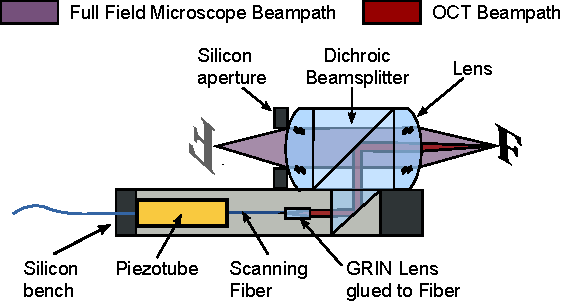
\includegraphics{figures/30_DesignSimulation/Overview/Schematic_paper.pdf}
      \caption{Schematic of the MEMS endomicroscope. Two glass lenses glued directly to the dichroic beamsplitter cube form the full field microscopy beam path. A silicon aperture is used to reduce the spherical aberrations. Buried beneath the full field optics, a single mode fiber glued to a collimating GRIN lens forms the OCT channel. The single-mode fiber is fixed in a piezoelectric tube to create a fiber scanner enabling 3D OCT. A reflecting micro-prism glued to a dichroic beamsplitter cube combines the two beam paths.}
      \label{fig:bimodalSketch}
\end{figure}

The base of the microbench with dimensions of $13 \times 2 \times \SI{1}{\milli\meter^3} $ is realized by standard silicon bulk micromachining. On the top layer, the bench accommodates the full field imaging optics that consists of a dichroic beamsplitter cube with dimensions of $2\times 2 \times  \SI{2}{\milli\meter^3}$ to separate the two beam paths and two plano-convex lenses with \SI{2}{\milli\meter} diameter, which form a full field microscope. To achieve a highly compact opto-mechanical design, the components of the OCT beam path are buried within a cavity in the base of the micro bench. On the bottom layer a gradient index lens (GRIN lens) with a diameter of \SI{350}{\micro\meter} is directly glued to the tip of a \SI{80}{\micro\meter} single mode fiber to collimate the infrared light of the OCT system with a center wavelength of $\lambda_o = \SI{1311}{\nano\meter}$ and a bandwidth of $\Delta \lambda = \SI{90}{\nano\meter} $. A spiral scanning of the OCT beam path is achieved by an angular scanner implemented using a piezoelectric tube actuator.

This actuator, called resonant fiber scanner, is able to scan a collimated beam by more than $\pm \SI{5}{\degree}$ by mechanically amplifying the subtle vibration of a piezoelectric actuator.  An objective lens focuses the beam on the tissue and transforms the angular displacement into a translation. By driving the scanner in two axes with two sinusoids at different phases, it is possible to sample a 2D area of the object in a spiral fashion, as explained in detail in Section \ref{sec:Optical}.

The rest of this chapter shows the design and development of the OCT imaging path for the multi-modal probe. However, in order to independently test the behavior of the OCT scanner and optics, a single modality probe was fabricated as a demonstrator. Both systems are mechanically and optically equivalent -- the only difference is the presence of the beam splitter. 
For completeness, both multi-mode and single-mode optical systems are described.


%%*****************************************************************************
\section{Optical Design of the OCT beam path}
\label{sec:Optical}
%%*****************************************************************************
This section explains in detail the design of the OCT optics and its scanning mechanism. Starting with the concept of a Fourier plane scanner, the most relevant design equations are derived, which guide the selection of the optical components to achieve the desired performance, eventually verified by optical simulation. 

\subsection{Fourier Plane Scanner}

%There are many reasons why this design is preferred over other scanning topologies. First, the narrow dimensions of the piezoelectric tube allow a compact implementation. Also, the field of view that can be achieved with this scanner is not limited to the space available for the GRIN lens to vibrate --- instead, to its maximum angular deflection. As we want a telecentric system, a \textit{4f} microscope could have been implemented instead of a Fourier plane scanner, but at the cost of duplicating the length of the optical system (Chapter \ref{Ch:Theory}). Another advantage of using a fourier plane scanner is that it requires a GRIN lens glued to the tip of the fiber in order to collimate the beam. As a side-effect, this extra weight greatly reduces the resonant frequency of the scanner, allowing a denser sampling from the data acquisition system. 


The OCT beam path is designed as an distal-side telecentric system to avoid distortions in the 3D OCT measurement. To achieve this, the fiber scanner is driven with small angles and is positioned such that the lateral and angular movement of the scanner imitates the beam angles that can be observed in the collimated region of a classical telecentric lens system. Figure \ref{fig:fps} illustrates this approach. The whole scanner is buried in a channel with a inner diameter of \SI{1}{\milli\meter} limiting the movement of the scanner to a maximum angle $\theta$ of \SI{5}{\degree} that allows a maximum FOV of \SI{1}{\milli\meter} of the OCT beam path.



\begin{figure}[h!]\centering 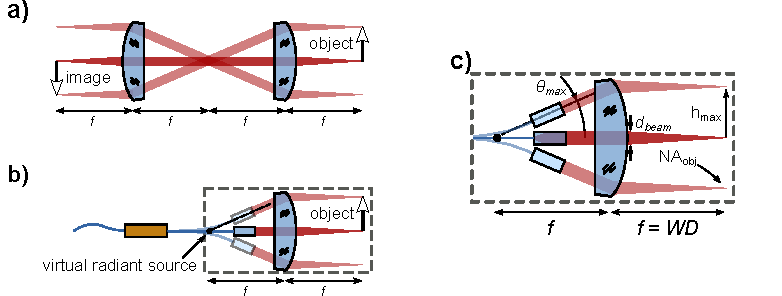
\includegraphics[width=\columnwidth]{figures/30_DesignSimulation/fps.pdf}
      \caption{\textbf{a)} Illustration of a classical telecentric system. The height of the object is translated into an angle $\theta$ in the collimated region between the two lenses. This angle is again translated into a corresponding image height by the second lens.
      \textbf{b)} Illustration of the OCT beam path using a fiber scanner in first resonance mode without micro prism and BS. The movement of the GRIN lens due to the fiber scanner and the distance between the GRIN lens and the focusing lens creating the same optical behavior as it can be observed in a classical object sided telecentric system. \\ \textbf{c)} Nomenclature used in this work.}
      \label{fig:fps}
\end{figure}

For the scanner to work as a Fourier plane scanner, at any point of the oscillation the output beam from the GRIN lens should point to a fixed virtual radiant source. This is fulfilled if the bending shape of the scanner is linear with the amplitude and thus, the ratio of the GRIN lens angle to its vertical displacement is kept constant $ y = d \cdot \tan \theta \simeq d \cdot \theta \Rightarrow \frac{\theta}{y} = const $ (refer to Figure \ref{fig:radiant}).

\begin{figure}[h!]\centering
      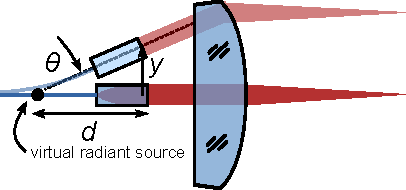
\includegraphics{figures/30_DesignSimulation/Mechanical/radiant.pdf}
      \caption{Schematic of the Fourier plane scanner at rest and at an arbitrary angle $\theta$. If the scanner behaves linearly, the output beam will appear to come from a fixed virtual radiant source regardless of the scanning amplitude.}
      \label{fig:radiant}
\end{figure}


In a Fourier plane scanner, the numerical apertures and focal lengths of the scanning and objective lens are related by the diameter of the beam in the intermediate region between both lenses. Thus, based on the schematic of Figure \ref{fig:fps}c, the following geometrical optics relations are obtained: $d_\mathrm{beam} \simeq 2\cdot f_\mathrm{GRIN}\cdot \mathrm{NA}_\mathrm{fiber}$ and $d_\mathrm{beam} \simeq 2 \cdot f_\mathrm{obj}\cdot \mathrm{NA}_\mathrm{OCT}$. By combining them together, the main design equation for the scanner follows:

\begin{equation}
f_\mathrm{GRIN} \cdot \mathrm{NA}_\mathrm{fiber} = f_\mathrm{obj} \cdot \mathrm{NA}_\mathrm{OCT}
\label{eq:fpsNA}
\end{equation}

Note that these equations use a small angle approximation valid for small NA: \\ $\tan[	\sin^{-1}(\mathrm{NA})] \simeq \mathrm{NA} $. In this case, as any NA is smaller than 0.25, the error of this simplification is smaller than 2\%.

\subsection{Component Selection}
The design equations that were obtained in the previous section relate all the optical components together. Therefore, once the desired NA is chosen, there is only a free variable available. In this case, the major constraint is given by the commercial availability of the single mode fiber, so the selection of the rest of the components will follow from it.

The only commercially available single mode fiber working in our wavelength range and with thinned cladding diameter (refer to Section \ref{sec:mechDesign}) is \textit{Thorlabs SM980G80}, with a diameter of \SI{80}{\micro\meter} and with $\mathrm{NA_\mathrm{fiber}} = 0.18$ at \SI{1.33}{\micro\meter}. 

In order to collimate the output from the fiber without clipping the gaussian beam, a GRIN lens with an $\mathrm{NA_{GRIN}}$ higher than $\mathrm{NA_{fiber}}$ is needed. A good fit from the GRINTECH catalog is \textit{GT-LFRL-035-024-20-CC (1550)}, with an $\mathrm{NA_\mathrm{GRIN}} = 0.20$ and $\mathit{f_\mathrm{GRIN}} = \SI{0.91}{\milli\meter}$. 

Now, by using the relation in \autoref{eq:fpsNA} we can design $f_\mathrm{objective}$ by choosing an adequate $\mathrm{NA_\mathrm{OCT}}$. To preserve a high depth of field (DOF), allow enough space for the beamsplitter and a long working distance, a narrow $\mathrm{NA_\mathrm{OCT}}$ is is preferred -- in the range of 0.020 - 0.025. By choosing an intermediate $\mathrm{NA_\mathrm{OCT}}$ of 0.022, the focal length of the objective lens 
\begin{equation}
\mathit{f_\mathrm{obj}} = f_\mathrm{GRIN}\ \frac{\mathrm{NA_\mathrm{fiber}}}{\mathrm{NA_\mathrm{OCT}}}  = \SI{0.91}{\milli\meter}\ \frac{0.18}{0.022} = \SI{7.5}{\milli\meter}
\end{equation}
can be selected. As one of the facets of the lens has to be cemented to the beamsplitter cube, it is fabricated as a plano-convex spherical lens by \textit{Optik+}.

The field of view (FOV) of the OCT modality can be now calculated considering the maximum angular deflection of the GRIN lens in the tip of the scanning fiber by 
\begin{equation}
h_\mathrm{max} = f_\mathrm{obj}\cdot \tan  \theta_\mathrm{max} = \SI{7.5}{\milli\meter} \cdot \tan \SI{5}{\degree} = \SI{0.66}{\milli\meter}, 
\end{equation}
equivalent to a FOV of \SI{1.2}{\milli\meter} for a $\theta_\mathrm{max} $ of $ \pm \SI{5}{\degree}$ (section \ref{sec:mechDesign}).


\subsection{ZEMAX Simulation}

Once the components are selected, it is possible to validate the theoretical analysis of the optical design by  performing a raytracing simulation. Using ZEMAX, the fiber facet is modeled as the waist of a gaussian beam source, the  GRIN lens is modeled using a design file from the manufacturer and the prism, beamsplitter and planoconvex lens are modeled geometrically according to the provided mechanical drawings. The result is shown in \autoref{fig:BS}.

\begin{figure}[h!]\centering
      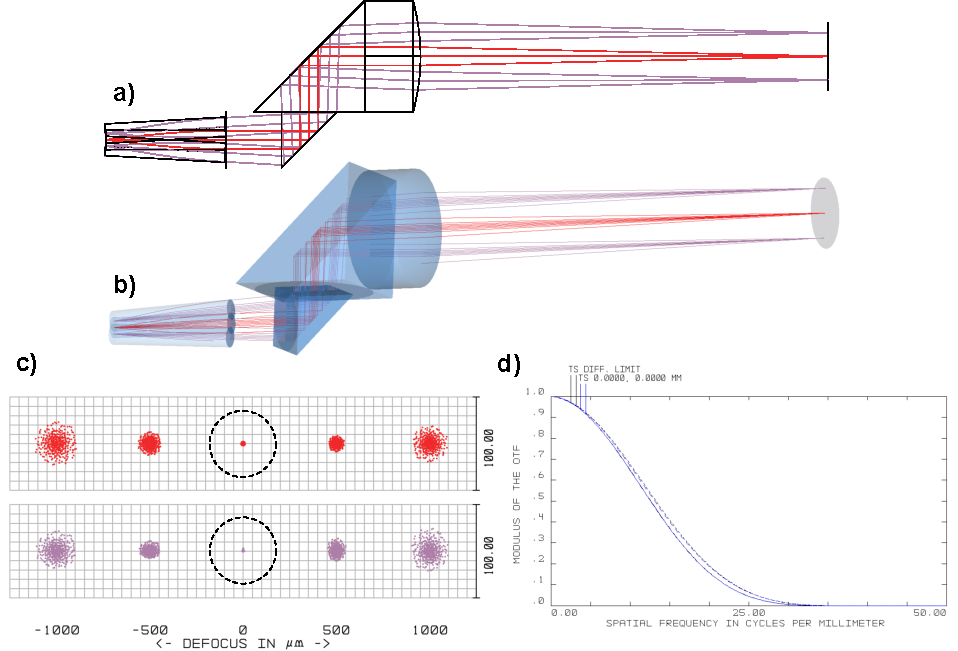
\includegraphics{figures/30_DesignSimulation/Optical/beamsplitterAll.pdf}
      \caption{\textbf{a)} 3D ZEMAX raytracing of the OCT beam path for the center (red rays) and marginal (purple rays) position of the GRIN lens. Note that as the OCT beam path is reflected in the hypotenuse of the beamsplitter, it can be modeled as a \SI{45}{\degree} prism.      
      \textbf{b)} Cross section of a) showing the most relevant dimensions.}
      \label{fig:BS}
\end{figure}

The three overlapping rectangles on the left simulate the rest position (red) and maximum deflection (purple) of the GRIN lens. The gap between GRIN lens and prism is calculated so that the focus of the planoconvex lens coincides with the virtual radiant source of the scanner.

	Due to the low $\mathrm{NA_\mathrm{OCT}}$ and the good optical quality of the GRIN and planoconvex lenses, the aberrations in this design are negligible and thus has an optical performance close to the diffraction limit. \autoref{fig:MTFsim} proves this behavior by comparing the MTF (Modulation Transfer Function) of an ideal optical system with the simulated MTF of the system which is described.

\begin{figure}[h!]\centering
      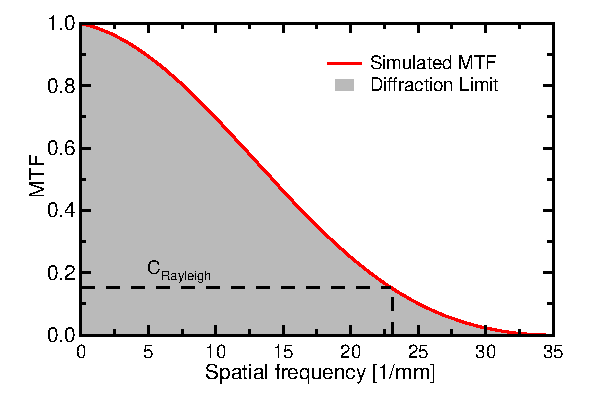
\includegraphics{figures/30_DesignSimulation/Optical/MTF/MTF_Sim.pdf}
      \caption{Simulated MTF curve of the OCT beam path for the bimodal probe. It can be seen that the system is diffraction limited and provides a lateral resolution of 23.3 lp/mm or \SI{43}{\micro\meter}.}
      \label{fig:MTFsim}
\end{figure}

\subsection{Minimization of backreflections}
%After the raytracing simulation of the optical system is performed, there is still an important factor to consider: the backreflections inside the probe. 
In OCT, any backreflection inside the probe increases the background intensity at the spectrometer, thus limiting its dynamic range. The consequences are higher noise, lower penetration depth and lower contrast of the resultant image. Therefore any source of backreflections in the design should be carefully considered and minimized. The main ones are marked in \autoref{fig:backreflections} and explained in the following list:

\begin{figure}[h!]\centering
      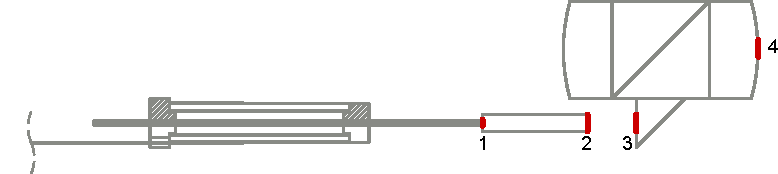
\includegraphics{figures/30_DesignSimulation/Optical/Backreflections/backreflections.pdf}
      \caption{Schematic of the multimodal probe showing the main interfaces where backreflections can originate inside the probe (red). 1) Fiber - GRIN. 2) GRIN - gap. 3) Gap - prism. 4) Objective - air. }
      \label{fig:backreflections}
\end{figure}

\begin{enumerate}

\item \textbf{Fiber - GRIN interface:}
Starting from the proximal side, the facet of the fiber and the GRIN lens are two parallel glass surfaces separated by a small gap. Although the beam is not collimated in this region, a small portion of light can be coupled back to the fiber. In order to minimize any backreflections, fiber and GRIN are glued together using a refractive-index-matched optical adhesive (\textit{NOA 76}, from \textit{Norland Products}). This way there is no glass to air interface and the maximum refractive index step is reduced to \SI{0.05}{}.
%Fiber 1.45670,NOA 1.51,GRIN 1.515 -> 275 ppm

\item \textbf{GRIN - gap interface:}
The next interface is the distal facet of the GRIN lens. This is a critical backreflection source -- regardless of the scanning angle, there is normal, collimated light incidence. To avoid this problem without resorting to delicate and expensive antireflection coatings, the GRIN lens is manufactured with a \SI{1}{\degree} tilt exit facet. According to geometrical optics, this tilt induces a vertical shift in the position of the backreflected focal point $\Delta y = f \tan(2\alpha)$ which in this system equates to $\SI{0.91}{\milli\meter} \cdot \tan (\SI{2}{\degree}) = \SI{31}{\micro\meter}$.

The result is visible in the simulation from \autoref{fig:tilt}: the backreflected light is focused back \SI{31}{\micro\meter} away, effectively missing the core of the fiber -- which has a diameter smaller than \SI{5}{\micro\meter}.

\begin{figure}[h!]\centering
      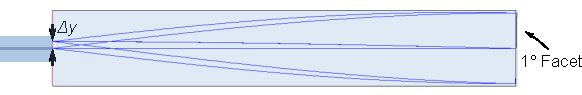
\includegraphics[width=10cm]{figures/30_DesignSimulation/Optical/backreflection.pdf}
      \caption{Schematic showing the raytracing simulation of a beam exiting from the distal facet of the fiber and being coupled into a GRIN lens with a tilted exit facet. Thanks to it, the backreflected light misses the core of the fiber and is thus not coupled back to the OCT system.}
      \label{fig:tilt}
\end{figure}

\item \textbf{Air - prism interface:} Due to collimated incidence, this interface can produce important backreflections, but only in the resting position of the GRIN lens, when the free end of the GRIN lens is pointing perpendicular to the surface of the prism. To minimize reflections in this situation it is possible to resort to anti-reflection coatings in the facet of the prism. 

\item \textbf{Objective lens - air interface:} After the prism, the beamsplitter and objective lens are cemented together, making any backreflections negligible. The objective lens has an interface with air, but has an anti-reflection coating on this surface. Furthermore, due to the curved surface of this lens, the backreflected light won't be focused back in the single mode fiber significantly.
\end{enumerate}

Taking these considerations into account, the backreflections were kept below 0.02\% in all the manufactured probes, as detailed in \autoref{ch:Results}.

\subsection{Single Modality Probe}
As stated in the Design Overview, in order to independently test the behavior of the OCT scanner and optics, a single modality probe was fabricated as a demonstrator. Its optical design, depicted in \autoref{fig:single}, emulates the multimodal design from \autoref{fig:BS} by unfolding its optical path. The main difference is the lack of the prism and beamsplitter and the orientation of the planoconvex lens, which has now with its convex surface facing the GRIN lens to reduce the backreflections which would happen in the case of normal incidence on the planar side of the lens.

\begin{figure}[h!]\centering
      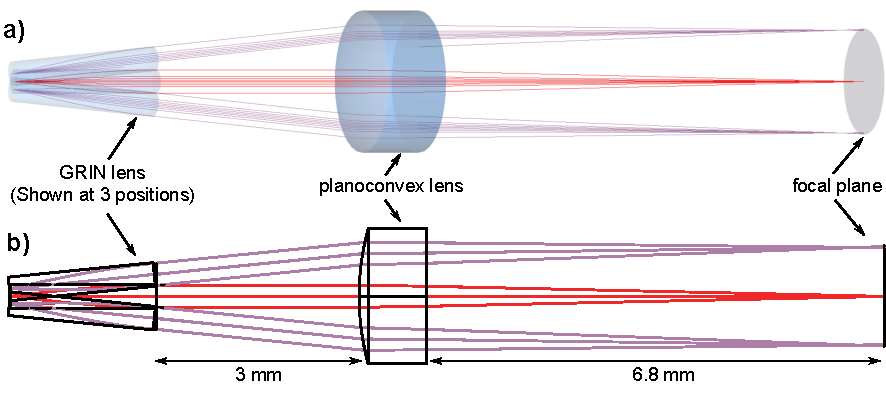
\includegraphics[width=12cm]{figures/30_DesignSimulation/Optical/singleAll.pdf}
      \caption{\textbf{a)} 3D ZEMAX raytracing of the OCT beam path for the center (red rays) and marginal (purple rays) position of the GRIN lens in the single modality demonstrator.
      \textbf{b)} Cross section of a).}
      \label{fig:single}
\end{figure}

The equivalence of both systems is emphasized by the similarity of their simulated MTF. Again, \autoref{fig:MTFcomp} indicates that the single modality demonstrator is diffraction-limited.

\begin{figure}[h!]\centering
      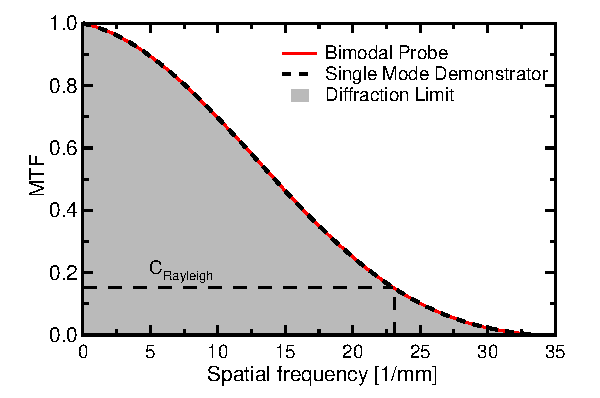
\includegraphics{figures/30_DesignSimulation/Optical/MTF/MTFComparison.pdf}
      \caption{Simulated MTF curve of the OCT beam path for the bimodal probe and the single modality demonstrator. It can be seen that both implementations are optically equivalent and diffraction limited, providing a lateral resolution of 23.3 lp/mm or \SI{43}{\micro\meter}.}
      \label{fig:MTFcomp}
\end{figure}

Due to these similarities, it is expected that any experimental result obtained with the demonstrator can be easily transferred to the behavior of the bimodal probe.

\subsection{Simulated Optical Performance}

To conclude the \textit{Design and Simulation} chapter, the most important characteristics of the components of the OCT microscope are listed in \autoref{tab:simChar} and the simulated performance in \autoref{tab:simRes}.

\begin{table}[h!]\centering
	\begin{tabular}{cc}\\
		\textbf{Parameter} & \textbf{Value} \\ 		
		\hline
     	\textbf{Single mode fiber NA} & 0.18 \\ 
		\textbf{GRIN lens NA} & 0.2 \\ 
		\textbf{GRIN lens focal length} & \SI{0.91}{\milli\meter} \\ 
		\textbf{Planoconvex lens focal length} & \SI{7.5}{\milli\meter} \\ 
		\hline
	\end{tabular}
		\caption{Summary of the most relevant characteristics of the optical components used in the OCT modality.}
\label{tab:simChar}
\end{table}

\begin{table}[h!]\centering
	\begin{tabular}{ccc}\\
		\textbf{Parameter} & \textbf{Bimodal Probe} & \textbf{Single Mode Demonstrator} \\ 
		\hline
		\textbf{Distal Side NA} & 0.022 & 0.022 \\ 
		\textbf{Working Distance} & \SI{7.3}{\milli\meter} &  \SI{6.8}{\milli\meter} \\ 
		\textbf{Field of View} & \SI{1.2}{\milli\meter} &  \SI{1.5}{\milli\meter}\\ 
		\textbf{Depth of Field} & \SI{3.4}{\milli\meter}& \SI{3.4}{\milli\meter} \\ 
		\textbf{Lateral Resolution} & \SI{43}{\micro\meter} & \SI{43}{\micro\meter}\\ 
		\hline
	\end{tabular} 
    \caption{Simulated optical performance and characteristics of the OCT modality. All resolution values follow the Rayleigh convention of 15.5\% modulation \cite{Kretschmer}.}
    \label{tab:simRes}
\end{table}

%%*****************************************************************************
\section{Image acquisition: Spiral Scanning}
\label{sec:spiralScanning}
%%*****************************************************************************

As described in the previous section, the OCT optical setup samples the object at only a single point. Thus, the focus point has to be 2D-scanned over the surface of the sample to obtain 3D OCT images.

A very compact solution to achieve this are resonant fiber scanners. These devices use the concept of mechanical resonance to amplify 100-fold the subtle movement of a piezoelectric actuator into a big displacement and angular deflection of the tip of a scanning fiber. 

As any resonant system, the movement of the scanning fiber is constrained to harmonic oscillations within a frequency close to its resonance frequency $f_\mathrm{res}$. This requirement constraints the possible scanning patters to harmonic movements at $f_\mathrm{res}$, excluding then  raster scanning, which require at least an axis working out of resonance. Then, conventional alternatives are Lissajous \cite{Moon2010} and spiral scanning. In order to ease the reconstruction of the image, this work implements the latter.

The following pages describe the concept of spiral scanning, its characteristics, limitations and implementation.

%%*****************************************************************************
\subsection{Driving and Acquisition}
%%*****************************************************************************
The piezoelectric tube which drives the scanner has four outer gold electrodes to control the lateral movement of the scanner, as described in \autoref{ch:theory}. Two independent voltage sources control the vertical and horizontal movement of the actuator by addressing the corresponding pair of electrodes. If sine and cosine signals of the same frequency $f_\mathrm{drive}$ are used to drive the scanner, the GRIN lens will oscillate in a circle of constant radius. If now the amplitude of these signals is modulated with another signal of frequency $f_\mathrm{mod}$, the resultant trajectory will be spiral, as illustrated in \autoref{fig:PZTDriving}.

\begin{figure}[h!]\centering 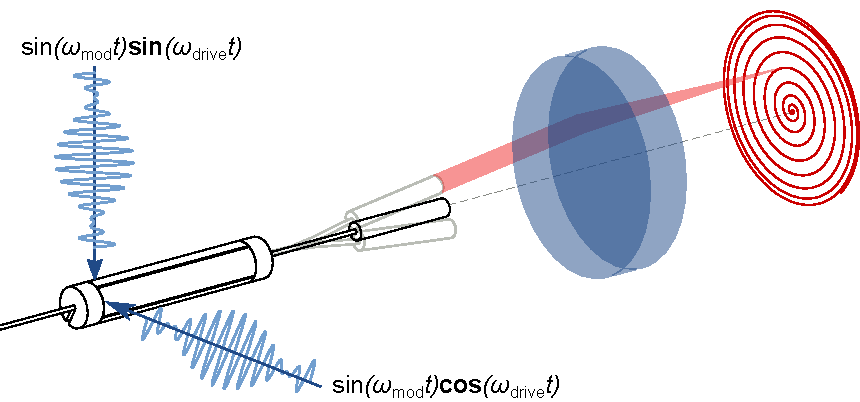
\includegraphics{figures/30_DesignSimulation/spiralScanning/PZTDrivingMoving.pdf}
      \caption{Schematic of the piezoelectric tube, fiber, GRIN and objective lens focusing the OCT beam (red) in a plane. 
      The piezoelectric tube is driven with two independent amplitude modulated sine and cosine signals to generate a spiral pattern, used to acquire an image. }
      \label{fig:PZTDriving}
\end{figure}

During the full period of the spiral pattern $T_\mathrm{spiral}=f_\mathrm{mod}^{-1}$ , two complete frames are acquired, one while the spiral grows, another while it shrinks. The whole pattern can be divided in $N_\mathrm{rings} = f_\mathrm{drive}/f_\mathrm{mod}$ individual rings, as depicted in \autoref{fig:spiralScanningNT}, each one acquired in a period $T_\mathrm{ring}=f_\mathrm{drive}^{-1}$. Thus the number of sample points that can be acquired in an individual ring
\begin{figure}[h!]\centering
      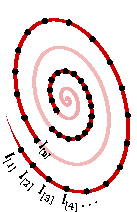
\includegraphics[width=4cm]{figures/30_DesignSimulation/spiralScanning/spiralScanningNT.pdf}
      \caption{Section of a spiral trajectory highlighting two different rings. The $n$ black dots represent the sampling points of each ring. Notice that in the inner ring the sampling density is higher than in the outer one.}
      \label{fig:spiralScanningNT}
\end{figure}
\begin{equation}
n = \frac{f_\mathrm{s}}{f_\mathrm{drive}}
\label{eq:nT}
\end{equation}
depends only on the driving frequency of the scanner $f_\mathrm{drive}$ and the sampling frequency $f_\mathrm{s}$ of the spectrometer, which is usually constant. This value is very important, as it defines the spatial sampling density. 

In order to fulfill the Nyquist theorem, the spacing between two adjacent sample points should be smaller than the Airy radius of the laser spot, . This condition is easily fulfilled in the inner rings of the spiral, as there the focus spot has a small speed, but as the radius of the spiral grows, so does the scanning speed and therefore the distance between sample points, as seen in \autoref{fig:spiralScanningNT}.

It is clear then that spiral scanning shows a non-uniform sampling distribution across the imaging field. Thus, to avoid undersampling in the outer areas, the number of samples per ring $n$ should be as high as possible. As OCT systems have a relatively small sampling frequency ($\sim$\SI{100}{\kilo\hertz}), the resonant frequency needs to be below \SI{1}{kHz} to achieve more than 100 acquired points per ring of the spiral.


%%*****************************************************************************
\section{Mechanical Design}
\label{sec:mechDesign}
%%*****************************************************************************
As explained in the previous section, in any resonant system, its geometrical and mechanical characteristics fully define the operating frequency range, and with it, constrain the way the final image can be sampled.

In the following paragraphs the behavior of the fiber scanner is mechanically modeled, and this information used to choose the most relevant fabrication parameters leading to an adequate resonant frequency for OCT.


\subsection{Resonance frequency calculation}
The scanner used in the probe consists of a piezoelectric tube which drives a beam composed of a single mode fiber and a GRIN lens into resonance, as depicted in \autoref{fig:EB}a.  

\begin{figure}[h!]\centering
      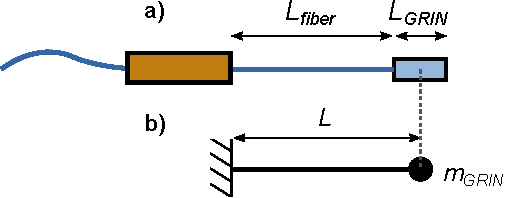
\includegraphics{figures/30_DesignSimulation/Mechanical/EB.pdf}
      \caption{\textbf{a)} Drawing of the piezoelectric scanner: piezoelectric tube, fiber and GRIN lens. 
      \textbf{b)} Simplified mechanical diagram obtained by modeling the fiber as a weightless cantilever and the GRIN lens as a point mass.}
      \label{fig:EB}
\end{figure}

The Euler-Bernoulli method can be used to estimate the resonant frequency of this scanner as detailed in \autoref{sec:EB}. Equations \ref{eq:EB} and \ref{eq:fres} show that there are several paths to reduce this frequency: increasing the cantilever length $L$, decreasing the radius of the fiber $r_\mathrm{fiber}$ or increasing the mass at the tip $m_{\mathrm{GRIN}}$. First, by having a GRIN lens attached at the tip, the resonance frequency is reduced by a factor of 62\%. Furthermore, by choosing a fiber with \SI{80}{\micro\meter} instead of the standard \SI{125}{\micro\meter}, the resonance frequency can be lowered by an extra factor of 60\%, as the sensitivity of the resonance frequency to the diameter of the fiber is quadratic. Under these conditions, the resonant frequency vs. length of the cantilever formed by a \SI{80}{\micro\meter} fused silica fiber with the chosen GRIN lens is computed in Figure \ref{fig:freq} using Equations \ref{eq:EB} and \ref{eq:fres}.

\begin{figure}[h!]\centering
      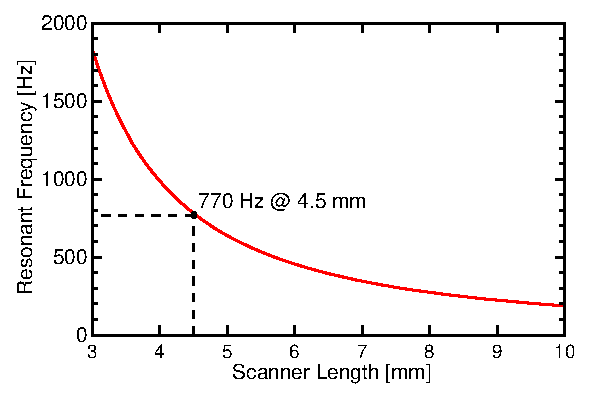
\includegraphics[width=10cm]{figures/30_DesignSimulation/Mechanical/fres/fres.pdf}
      \caption{Resonant frequency of the scanner as a function of the total scanning tip length ($L_\mathrm{fiber} + L_\mathrm{GRIN}$). The chosen working point is labeled in the plot.}
      \label{fig:freq}
\end{figure}

In order to select the length of the scanner there are two things to consider. As the scanner is buried in a \SI{1}{\milli\meter} channel, the maximum displacement of the GRIN lens is limited to $\pm\SI{325}{\micro\meter}$. Within that small displacement we want to achieve the maximum angular deflection of the GRIN lens to maximize the FOV, what can be achieved by using shorter fiber lengths. This shows a trade-off with the density of sampling $N_\mathrm{T}$, which is increased with longer fiber lengths. To balance those terms, we chose a a total scanner length of \SI{4.5}{\milli\meter}, which fulfills all the before-mentioned requirements, as \autoref{tab:mech} shows. 

\begin{table}[h!]\centering
	\begin{tabular}{rl}\\
		\hline
		\textbf{Cantilever length} & \SI{4.5}{\milli\meter} \\ 
		\textbf{Resonant Frequency} & \SI{770}{\hertz} \\ 
		\textbf{Max. angular deflection} & \SI{5}{\degree} \\ 
		\hline
	\end{tabular} 
    \caption{Mechanical characteristics of the fiber scanner at its designed working point.}
    \label{tab:mech}
\end{table}

\subsection{COMSOL simulation}

In order to validate the theoretical analysis of the previous section, a multiphysics finite element analysis was performed using \textit{COMSOL}. For that matter, the actuator was modeled as a radially polarized piezoelectric material (\textit{PIC 151}) and the rest of the structure as fused silica. The excitation voltage is a sinusoidal symmetrical potential between the top and bottom electrodes of the tube. Note that, as the system undergoes small deflections, it is simulated assuming linear behavior \cite{Fertis2006} without incurring in important deviations.

As the first step, the resonant frequency of the system is simulated. An Eigenfrequency study calculates the first mode resonance at \SI{762}{\hertz}, which closely matches the analytical estimation of \SI{770}{\hertz}. The mode shape at resonance is shown in Figure \ref{fig:defle}, where it can be observed that the actuator and the base of the fiber are almost static, confirming the resonant behavior of the scanner.

\begin{figure}[h!]\centering
      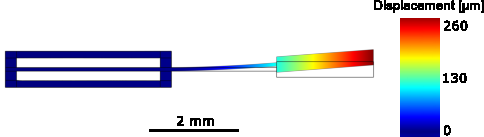
\includegraphics[width=10 cm]{figures/30_DesignSimulation/Mechanical/deflection.pdf}
      \caption{COMSOL simulation showing a cross section of the scanner maximum deflection at resonance. The deformed structure is color coded showing the total displacement from the rest position (shown outlined). }
      \label{fig:defle}
\end{figure}

%Note that, as the system is working at its resonance, it is very difficult to simulate the oscillation amplitude, as it depends on its damping factor which should be obtained experimentally. Thus, for the simulation, this value was chosen to fit the expected deflection. 

Thanks to the multiphysics simulation, it is also possible to check the electric field distribution inside the piezoelectric tube. As can be seen in Figure \ref{fig:field}, for a symmetrical actuation in the top and bottom electrodes with a voltage of $\pm \SI{75}{\volt}$, most of the volume under these electrodes experiences a field magnitude close to the expected theoretical value $E=U/d = \SI{75}{\volt}/\SI{150}{\micro\meter} = \SI{500}{\volt/\meter}$, which is under the safe operating field of \textit{PIC 151}, ranging from $ +\SI{1000}{\volt/\meter}$ to $ -\SI{700}{\volt/\meter}$. Only some fringe areas exceed these values, which could become depolarized with time.
\begin{figure}[h!]\centering
      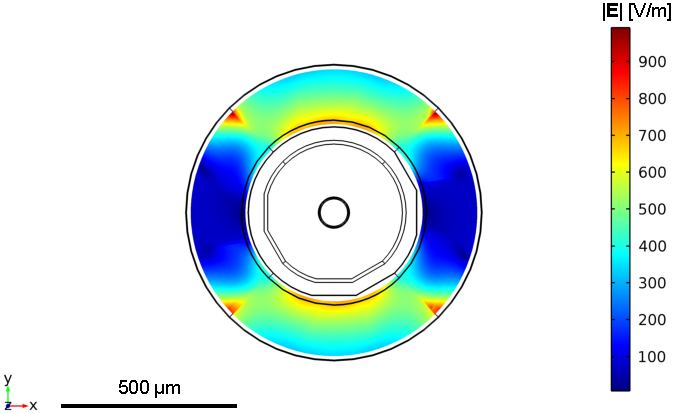
\includegraphics{figures/30_DesignSimulation/Mechanical/field.pdf}
      \caption{Magnitude of the electrical field inside a cross-section of the piezoelectric tube with an excitation voltage of $\pm \SI{75}{\volt}$ applied to the top and bottom electrodes.}.
      \label{fig:field}
\end{figure}
      
      
